\documentclass[11pt]{article}

% Generated by tools/author/maptex.py. Do not edit; edit the map's author script
% and run it again.

\usepackage[T1]{fontenc}
\usepackage[utf8]{inputenc}
\usepackage[margin=0.85in]{geometry}
\usepackage{amsmath}
\usepackage{kpfonts}
\usepackage{tikz}
\usetikzlibrary{arrows.meta}
\usepackage{enumitem}
\usepackage{multicol}
\usepackage{xcolor}

\definecolor{maroon}{HTML}{800000}
\definecolor{inkgrey}{HTML}{4D4D4D}

\pagestyle{empty}
\setlength{\parindent}{0pt}

\newcommand{\heading}[1]{%
  \par\medskip{\large\bfseries\color{maroon} #1}\par\smallskip}

\tikzset{
  concept/.style={rectangle, draw=inkgrey, rounded corners=2pt,
    align=center, font=\footnotesize, inner sep=3pt, fill=white, line width=0.5pt},
  edgenum/.style={circle, fill=white, draw=inkgrey, inner sep=0pt,
    minimum size=11pt, font=\scriptsize\bfseries, line width=0.4pt},
  nlabel/.style={font=\tiny\bfseries, text=inkgrey, inner sep=1pt},
  % One style for every arrow. Which of the four kinds it is is part of the
  % question, so the drawing must not answer it.
  arr/.style={-, thick, inkgrey},
  solved/.style={-{Latex[length=2mm]}, thick, maroon},
}

\begin{document}

{\LARGE\bfseries\color{maroon} Sequences and series of functions}\par\medskip
{\color{inkgrey}\small Math 163 \quad\textbullet\quad Prof.\ Chowdhury \quad\textbullet\quad Concept map}\par\bigskip

The next page shows 14 ideas as labelled boxes, joined by 15 numbered arrows. Every arrow is a real mathematical relationship, and the drawing does not tell you which kind: an arrow may \emph{hold}, it may \emph{fail}, the two ideas may be \emph{equivalent}, or it may hold on \emph{other hypotheses} than the ones its neighbours use. For each numbered arrow, circle the kind and describe the relationship in one sentence. Name the theorem, state the hypothesis that is doing the work, or say what goes wrong.

\heading{What each box means}
\small
\begin{enumerate}[label=\textbf{\Alph*.}, leftmargin=2.2em, itemsep=1pt]
\item \textbf{Pointwise Convergence.} For each \(x\) and each \(\varepsilon > 0\) there is an \(N\) depending on both, with \(|f_n(x) - f(x)| < \varepsilon\) for \(n \ge N\).
\item \textbf{Uniform Convergence.} For each \(\varepsilon > 0\) there is an \(N\) depending only on \(\varepsilon\), with \(|f_n(x) - f(x)| < \varepsilon\) for \(n \ge N\) and every \(x\) at once.
\item \textbf{Cauchy Criterion.} \(\{f_n\}\) converges uniformly exactly when for each \(\varepsilon > 0\) there is an \(N\) with \(|f_m(x) - f_n(x)| < \varepsilon\) for all \(m, n \ge N\) and all \(x\).
\item \textbf{Continuity of Limit.} Each \(f_n\) continuous and \(f_n \to f\) uniformly gives \(f\) continuous.
\item \textbf{Integrability of Limit.} Each \(f_n\) integrable and \(f_n \to f\) uniformly gives \(f\) integrable, with \(\lim \int f_n = \int \lim f_n\).
\item \textbf{Differentiability of Limit.} \(f_n \to f\) pointwise together with \(f_n' \to g\) uniformly gives \(f' = g\). It is the derivatives that have to converge uniformly.
\item \textbf{Dini's Theorem.} \(f_n \to f\) pointwise on \([a,b]\), monotonely, with every \(f_n\) and \(f\) continuous, gives \(f_n \to f\) uniformly.
\item \textbf{Series of Functions \(\sum f_n\).} \(\sum f_n\) converges when its partial sums \(S_N(x) = \sum_{k \le N} f_k(x)\) do. A series of functions is a sequence of functions.
\item \textbf{Weierstrass \(M\)-test.} If \(|f_n(x)| \le M_n\) for every \(x\) and \(\sum M_n < \infty\), then \(\sum f_n\) converges uniformly and absolutely.
\item \textbf{Power Series \(\sum a_n(x-c)^n\).} A series of functions whose \(n\)th term is a monomial of degree \(n\) centred at \(c\).
\item \textbf{Radius of Convergence \(R\).} \(\sum a_n(x-c)^n\) converges absolutely for \(|x - c|  R\). The endpoints are checked one at a time.
\item \textbf{Term-by-term Diff. and Integ..} Inside \((c-R, c+R)\) a power series can be differentiated and integrated term by term, and the result has the same radius \(R\).
\item \textbf{Taylor Series.} \(\sum f^{(n)}(a)(x-a)^n/n!\). The coefficients are forced by differentiating the power series at its centre.
\item \textbf{Taylor series converges to \(f\).} The Taylor series converges to \(f(x)\) exactly when the remainder \(R_N(x) = f(x) - P_N(x)\) tends to zero.
\end{enumerate}
\normalsize
\heading{Examples worth keeping to hand}
\small
\begin{itemize}[leftmargin=1.4em, itemsep=1pt]
\item \(x^n\) on \([0,1]\) takes continuous functions to a discontinuous limit, pointwise.
\item \(\sqrt{x^2 + 1/n^2} \to |x|\) uniformly, and the limit is not differentiable at \(0\).
\item \((1/n)\sin(n^2x) \to 0\) uniformly while its derivatives diverge.
\item \(x/(1 + n^2x^2) \to 0\) uniformly, and the derivative of the limit is not the limit of the derivatives at \(0\).
\item \(e^{-1/x^2}\) extended by \(0\) is infinitely differentiable at \(0\) with every Taylor coefficient zero, so its Taylor series converges and not to it.
\end{itemize}
\normalsize
\newpage
\vspace*{\fill}
\begin{center}
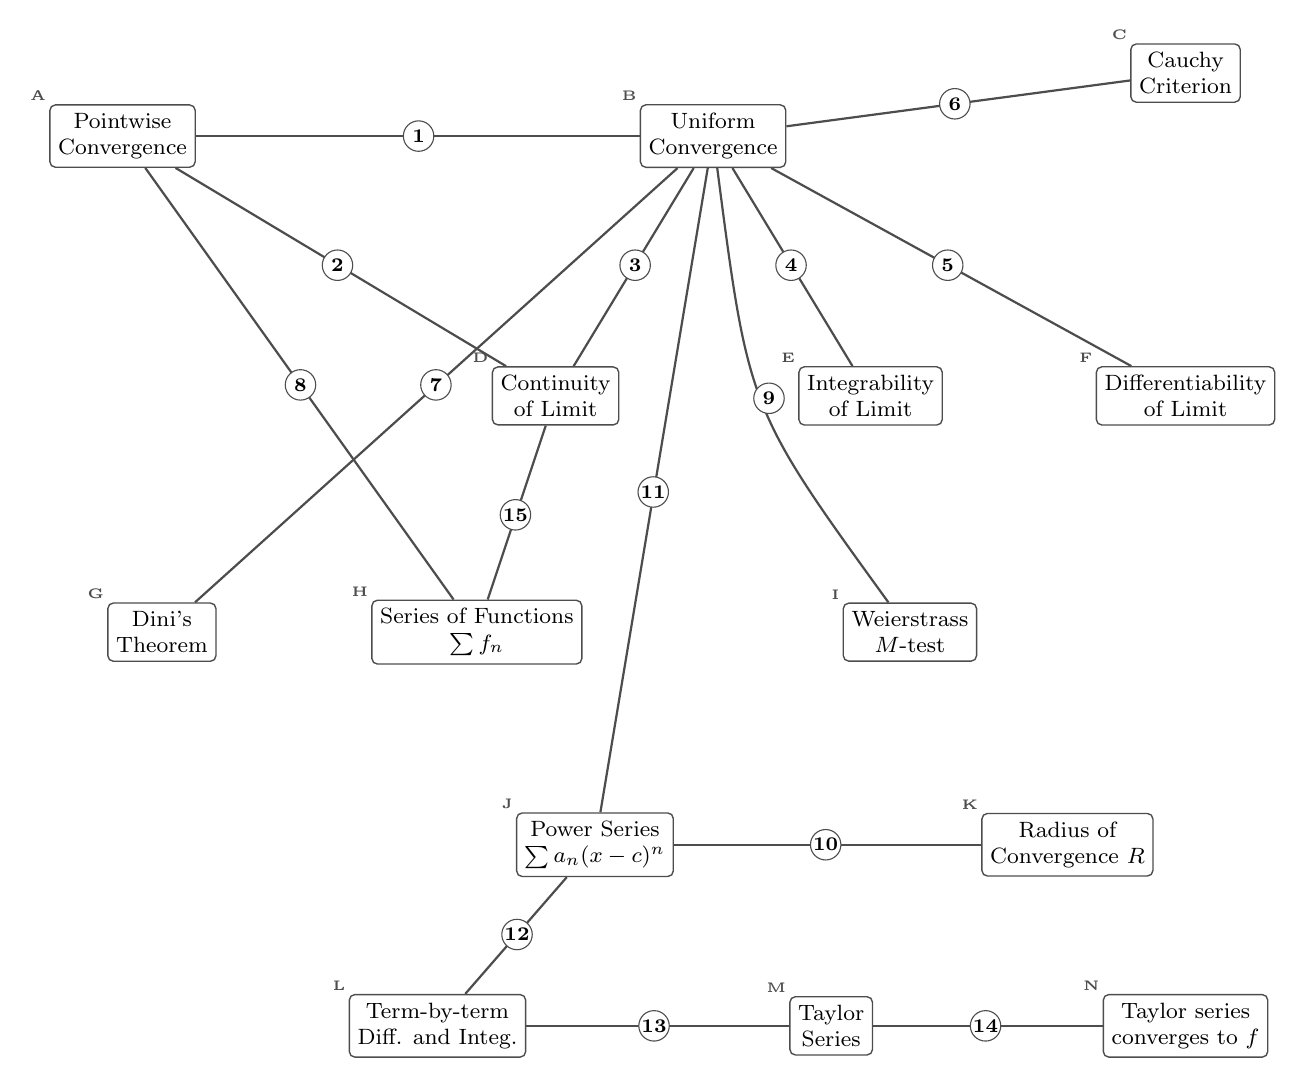
\begin{tikzpicture}[>=Latex]
  \node[concept] (A) at (-6, 0) {Pointwise \\ Convergence};
  \node[concept] (B) at (1.5, 0) {Uniform \\ Convergence};
  \node[concept] (C) at (7.5, 0.8) {Cauchy \\ Criterion};
  \node[concept] (D) at (-0.5, -3.3) {Continuity \\ of Limit};
  \node[concept] (E) at (3.5, -3.3) {Integrability \\ of Limit};
  \node[concept] (F) at (7.5, -3.3) {Differentiability \\ of Limit};
  \node[concept] (G) at (-5.5, -6.3) {Dini's \\ Theorem};
  \node[concept] (H) at (-1.5, -6.3) {Series of Functions \\ \(\sum f_n\)};
  \node[concept] (I) at (4, -6.3) {Weierstrass \\ \(M\)-test};
  \node[concept] (J) at (0, -9) {Power Series \\ \(\sum a_n(x-c)^n\)};
  \node[concept] (K) at (6, -9) {Radius of \\ Convergence \(R\)};
  \node[concept] (L) at (-2, -11.3) {Term-by-term \\ Diff. and Integ.};
  \node[concept] (M) at (3, -11.3) {Taylor \\ Series};
  \node[concept] (N) at (7.5, -11.3) {Taylor series \\ converges to \(f\)};

  \node[nlabel, anchor=south east] at (A.north west) {A};
  \node[nlabel, anchor=south east] at (B.north west) {B};
  \node[nlabel, anchor=south east] at (C.north west) {C};
  \node[nlabel, anchor=south east] at (D.north west) {D};
  \node[nlabel, anchor=south east] at (E.north west) {E};
  \node[nlabel, anchor=south east] at (F.north west) {F};
  \node[nlabel, anchor=south east] at (G.north west) {G};
  \node[nlabel, anchor=south east] at (H.north west) {H};
  \node[nlabel, anchor=south east] at (I.north west) {I};
  \node[nlabel, anchor=south east] at (J.north west) {J};
  \node[nlabel, anchor=south east] at (K.north west) {K};
  \node[nlabel, anchor=south east] at (L.north west) {L};
  \node[nlabel, anchor=south east] at (M.north west) {M};
  \node[nlabel, anchor=south east] at (N.north west) {N};

  \draw[arr] (B) .. controls (-2.25, 0.00) .. (A);
  \draw[arr] (A) .. controls (-3.25, -1.65) .. (D);
  \draw[arr] (B) .. controls (0.50, -1.65) .. (D);
  \draw[arr] (B) .. controls (2.50, -1.65) .. (E);
  \draw[arr] (B) .. controls (4.50, -1.65) .. (F);
  \draw[arr] (C) .. controls (4.50, 0.40) .. (B);
  \draw[arr] (G) .. controls (-2.00, -3.15) .. (B);
  \draw[arr] (H) .. controls (-3.75, -3.15) .. (A);
  \draw[arr] (I) .. controls (1.95, -3.47) .. (B);
  \draw[arr] (J) .. controls (3.00, -9.00) .. (K);
  \draw[arr] (J) .. controls (0.75, -4.50) .. (B);
  \draw[arr] (J) .. controls (-1.00, -10.15) .. (L);
  \draw[arr] (L) .. controls (0.50, -11.30) .. (M);
  \draw[arr] (M) .. controls (5.25, -11.30) .. (N);
  \draw[arr] (H) .. controls (-1.00, -4.80) .. (D);

  \node[edgenum] at (-2.24, -0.00) {1};
  \node[edgenum] at (-3.27, -1.64) {2};
  \node[edgenum] at (0.51, -1.64) {3};
  \node[edgenum] at (2.49, -1.64) {4};
  \node[edgenum] at (4.48, -1.64) {5};
  \node[edgenum] at (4.57, 0.41) {6};
  \node[edgenum] at (-2.02, -3.16) {7};
  \node[edgenum] at (-3.74, -3.16) {8};
  \node[edgenum] at (2.21, -3.33) {9};
  \node[edgenum] at (2.93, -9.00) {10};
  \node[edgenum] at (0.74, -4.52) {11};
  \node[edgenum] at (-0.99, -10.14) {12};
  \node[edgenum] at (0.75, -11.30) {13};
  \node[edgenum] at (4.96, -11.30) {14};
  \node[edgenum] at (-1.01, -4.81) {15};
\end{tikzpicture}
\end{center}
\begin{center}\small\color{inkgrey}
Every arrow is drawn the same way. For each one, decide whether it holds, fails, is an equivalence, or holds on other hypotheses, and say what it claims.
\end{center}
\vspace*{\fill}
\newpage
\heading{The arrows}
\small
\begin{multicols}{2}
\begin{enumerate}[label=\textbf{\arabic*.}, itemsep=0.55em, leftmargin=1.8em]
\item
  {\scriptsize\color{inkgrey} holds \;/\; fails \;/\; equivalent \;/\; other hypotheses}\par\vspace{2pt}
  \dotfill\\[2pt]\dotfill
\item
  {\scriptsize\color{inkgrey} holds \;/\; fails \;/\; equivalent \;/\; other hypotheses}\par\vspace{2pt}
  \dotfill\\[2pt]\dotfill
\item
  {\scriptsize\color{inkgrey} holds \;/\; fails \;/\; equivalent \;/\; other hypotheses}\par\vspace{2pt}
  \dotfill\\[2pt]\dotfill
\item
  {\scriptsize\color{inkgrey} holds \;/\; fails \;/\; equivalent \;/\; other hypotheses}\par\vspace{2pt}
  \dotfill\\[2pt]\dotfill
\item
  {\scriptsize\color{inkgrey} holds \;/\; fails \;/\; equivalent \;/\; other hypotheses}\par\vspace{2pt}
  \dotfill\\[2pt]\dotfill
\item
  {\scriptsize\color{inkgrey} holds \;/\; fails \;/\; equivalent \;/\; other hypotheses}\par\vspace{2pt}
  \dotfill\\[2pt]\dotfill
\item
  {\scriptsize\color{inkgrey} holds \;/\; fails \;/\; equivalent \;/\; other hypotheses}\par\vspace{2pt}
  \dotfill\\[2pt]\dotfill
\item
  {\scriptsize\color{inkgrey} holds \;/\; fails \;/\; equivalent \;/\; other hypotheses}\par\vspace{2pt}
  \dotfill\\[2pt]\dotfill
\item
  {\scriptsize\color{inkgrey} holds \;/\; fails \;/\; equivalent \;/\; other hypotheses}\par\vspace{2pt}
  \dotfill\\[2pt]\dotfill
\item
  {\scriptsize\color{inkgrey} holds \;/\; fails \;/\; equivalent \;/\; other hypotheses}\par\vspace{2pt}
  \dotfill\\[2pt]\dotfill
\item
  {\scriptsize\color{inkgrey} holds \;/\; fails \;/\; equivalent \;/\; other hypotheses}\par\vspace{2pt}
  \dotfill\\[2pt]\dotfill
\item
  {\scriptsize\color{inkgrey} holds \;/\; fails \;/\; equivalent \;/\; other hypotheses}\par\vspace{2pt}
  \dotfill\\[2pt]\dotfill
\item
  {\scriptsize\color{inkgrey} holds \;/\; fails \;/\; equivalent \;/\; other hypotheses}\par\vspace{2pt}
  \dotfill\\[2pt]\dotfill
\item
  {\scriptsize\color{inkgrey} holds \;/\; fails \;/\; equivalent \;/\; other hypotheses}\par\vspace{2pt}
  \dotfill\\[2pt]\dotfill
\item
  {\scriptsize\color{inkgrey} holds \;/\; fails \;/\; equivalent \;/\; other hypotheses}\par\vspace{2pt}
  \dotfill\\[2pt]\dotfill
\end{enumerate}
\end{multicols}
\normalsize
\heading{One last question}
Which single arrow carries the most of this chapter? Say why in one sentence. If your answer is the one arrow whose hypotheses are not what you expected, say what you expected instead.
\par\medskip\dotfill\\[4pt]\dotfill\\[4pt]\dotfill

\vfill
{\scriptsize\color{inkgrey} Contents by Subhadip Chowdhury, licensed CC BY-NC-SA 4.0. Built with AI assistance; the mathematics was checked by a human.\par}
\end{document}
